\documentclass[9pt,a4paper]{acmproc}
\usepackage[utf8]{inputenc}
\usepackage{amsmath}
\usepackage{amsfonts}
\usepackage{amssymb}
\usepackage{graphicx}
\usepackage[english]{babel}
\usepackage[utf8]{inputenc}
\usepackage{amsmath}
\usepackage{cite}
\usepackage{afterpage}


\graphicspath{}

\author{
\texttt{Andreas Nordberg}\\
\texttt{andno793@student.liu.se}
  \and
  \texttt{Jonathan Sjölund}\\
  \texttt{jonsj507@student.liu.se}
}

\begin{document}


\title{%
	Geo-based media player \\
	\large An interactive interface for geo-based video streaming}
\maketitle

%%Ta bort två sidor
\cleardoublepage
\pagenumbering{arabic}
\setcounter{page}{3}

\begin{abstract}
Being able to interact with a video stream can be both fun and educational however, to achieve the best user experience, the interaction must be seamless. Creating a media player that can allow users to view a video stream from different geographical positions is a challenge that is tackled in this paper. This paper describes the material and methods used to accomplish this kind of media player. And it explains how to achieve a seemingly good and, to higher extent, enjoyable video streaming experience. A proof-of-concept is shown of a mediaplayer that enables a user to see an overview over a geographical streaming location. By seeing each streams relative location to the point-of-interest the users are able to click on that stream and switch to it in a seamless way. It is shown that it is possible to switch between most nearby videos without interrupting or impairing the video streaming experience. (This is not final or necessary correct but hopefully something we can accomplish)

\end{abstract}

\begin{keywords}
HTTP Adaptive Streaming (HAS), OSMF video player, Interactive video streaming, Geographical based streaming (GBS), Seamless playback
\end{keywords}

\section{Introduction} 

Streaming has evolved and become more popular over last couple of years. Thousands upon thousands of different streams are being watched every day\footnote{Twitch statistics https://stats.twitchapps.com/, Fetched: 2016-04-01}, thus the demand for better and more ways to stream are longed for. If we could stream videos in different ways we can create a more interesting streaming environment, this can provide both better entertainment but also a better way to potentially improve observation in science and other areas more reliably. If a stream can provide the possibility for watching a video from different angles it can give people the option to observe and also enjoy something from different perspectives. This project focuses on accomplishing that, by creating a geo-based video player that uses HTTP-adaptive streaming (HAS) that can allow people to view a video from different angles and change between them seamlessly without any buffering delay or stuttering. By looking at an existing video streaming player and improve it to accomplish this task we show that it is something worth implementing in already existing media players.

In this project we design and develop a geo-based command-and-control video streaming player using geo-tags. In practice this means that a service in which you can choose between a set of recording streams of the same event, for example, but slightly different locations and angles. This would be a useful feature to have in any larger event where you would want to show the same scene from different locations and angles. The interface will be useful for both event-organizers that hire staff to make several different recordings of the same scene for simultaneous viewing, but could also be used by the public who volunteer to record the event live.

\subsection{Boundaries}
The application we provide is only going to be a proof-of-concept which means that we will only focus on the functionality of the video player. Factors like a pretty interface and usability on broader spectrum will be neglected. We will focus on making the application work for only one user to verify the functionality we want to accomplish. The number of video streams that we will be able to seamlessly switch between will,for the purpose of testing, be limited to a few, but then expanded upon to support any reasonable number of streams. This is because we firstly want to make sure that it is possible to switch between video streams and not that it can be done over large numbers. The reason for this is that pre-buffering many videos can be difficult to accomplish with a large number of video streams. As long as we provide a way to do it the solution can be expanded upon.


\section{Background and Related Work}
To be able to grasp the concept of how HTTP-adaptive streaming (HAS) and geo-based streaming (GBS) works we first present background on HAS and GBS in order to further strengthen our methodology and the interpretation of our result. Since we are using HAS and GBS when programming our interface there is a need to study existing works and articles. By using that knowledge it becomes possible to implement a new upgraded media player that is adapted to streaming from different geographical positions.

There are many related works to our work. Many of these works are focusing on branching videos in media players, which describes ways to allow for users to seamlessly switch between videos without quality degradation or interruptions \cite{qualbranch, hasmultipath,scalableOnDemand}. Zhao et al. \cite{scalableOnDemand} propose protocols that enables the possibility of scaleable on-demand content with minimal server load and developing a way that limits the lower bound bandwidth requirement using multicast \cite{scalableOnDemand}. Other works talks about policies for providing a good way of prefetching several videos in different ways, providing means of allowing prefetching and instantaneous playback without playback quality degradation. The work studies the off-periods observed in HAS-players to utilize it as effectively as possible \cite{bandawarePrefetch}.

There are also works that have looked at optimiziation of video quality by observing and controlling the playback buffer by in turn looking at the network capacity, providing an algorithm for optimizing the video quality without any unnecessary buffering \cite{bufferbased}.

\subsection{HTTP-based Adaptive Streaming}
Mobile users streaming media sometimes suffers from playback interruption when faced with a bad wireless connection. HTTP-adaptive streaming seeks to resolve this by dynamically changing the bitrate and therefore quality of the stream to make do with the connection that is available to the user. To ensure smooth transitions between these quality swaps HAS also tries to predict the swaps in advance using various methods depending on the HAS framework. There are many algorithms for these predictions, but a brief example would be to use previous logged connectivity history and future connectivity using geo-based methods to make predictions \cite{gtube}. Most HAS players uses weighted average of past download time/rates in order to estimate download rate of available bandwidth \cite{qualbranch}. With these HAS predictions, a stream quality fitting the user’s network quality can be buffered \cite{gtube}.

With HAS-adaptive streaming it is needed for us to prefetch data from several close-by streams (if not all, depending on number of them) and build up a small enough buffer that makes switching between different streams seamless. By looking at how HAS is used when implementing an interactive branched video we can say that parallel TCP connections is a must in-order to achieve this with a cost of wasting bandwidth and lower playback quality. This depends mainly on the number of videos that needs to be prefetched. Most HAS video players has a cap on the buffer size in order to avoid wasting bandwidth. Krishnamoorthi et al. \cite{qualbranch} use a customized HAS player that solves the problem of trade-off between quality and number of chunks downloaded. The playback chunks are stored in the playback buffer while the prefetched chunks are stored in a browser cache thus allowing those chunks to be retrieved quickly. This ensures that no playback interruption occurs for the user. The way they download the chunks are done in a round-robin way to ensure that a buffer workahead is built up enough for seamless playback in parallel TCP downloading. 

Downloading chunks in a round-robin way is how chunks will be downloaded in our media player. This way will be used together with the idea of prefetching in the downtime of a HAS-player. Most HAS-players has some kind of buffer treshold $T_{max}$ where downloading is interrupted when reached and will resume only when the minimum buffer $T_{min}$ is reached. This kind of behaviour can be called an \textit{on-off behaviour} which can lead to poor performance under conditions with competing traffic. It is common in several HAS-players like Netflix and Microsoft Smooth Streaming for example. Krishnamoorthi et al. \cite{bandawarePrefetch} provide policies and ideas that reduce the start-up time of videos by an order of magnitude and ensures the highest possible playback quality to be viewed. A way of improved channel utilization that allows for instantaneous playback of prefetched videos. They provide an HAS solution which we will take advantage of together with prefecthing nearby streams in a round-robin way. The solution allows for prefetching and buffer management in such a way that videos can be downloaded parallel and switched to instantaneous without interrupting the user experience. By using a novel system to utilize the unused bandwidth during off periods this allows for videos to simultaneously be prefetched while maintaining a fair bandwidth share. It also increases the playback quality in which a video is downloaded \cite{bandawarePrefetch}. This idea will be discussed further in section 2.2 when we describe our idea of downloading streams.

There can occur several problems in HAS players \cite{qualbranch}. Huang et al. \cite{streamrate} show that when a competing TCP flow starts a so called “downward spiral effect” occurs and the downgrade in throughput and playback rate becomes severe. This is caused by a timeout in the TCP congestion window, high packet loss in competing flows and when a client has a lower throughput the playback rate is lower due to smaller buffer segments which makes a video flow more susceptible to perceiving lower throughput and thus creating a spiral. A possible solution is to have larger segment size and by having an algorithm which is less conservative, meaning that requesting a video at lower rate than is perceived. This is something that we can keep in mind since quality can decrease drastically when having several videos buffering in parallel, though we will not have to buffer a full video at the same time but only chunks of a video while the main stream is being watched.

\subsection{Non-linear Streaming and Multipath}
Krishnamoorthi et al. \cite{hasmultipath} use this technique of storing prefetched chunks in a playback buffer simliar to [6]. Prefetching for different branches to allow seamless switching between videos, using the notion of multi-path nonlinear videos to stitch together videos using a novel buffer management and prefetching policy. This prefetching decreases the time it takes to switch between branches considerably and is something we will take advantage of since the code we use from \cite{qualbranch} are based on a similar policy \cite{hasmultipath}. If we look at \textit{Scalable On-Demand Streaming of 
Nonlinear Media} they describe how choosing a correct branching point sufficiently ahead of time with an accuracy of 75 \% greatly reduces bandwidth requirements. Requesting nonlinear video content where chunks are downloaded parallel without causing jitter. This is something which is really important and efficient for users that would like the ability to switch between different videos on-demand. Selecting what type of chunks should be downloaded is hard to accomplish, atleast on a broader context when considering watching TV stream during TV broadcasting \cite{scalableOnDemand}.  Most of these works are mostly focused on branching videos which is simliar but not entierly simliar to what we will be doing \cite{qualbranch, hasmultipath,scalableOnDemand}. We will contribute more to the possibility of prefetching several videos parallel and then be able to switch to any of  them on-demand. However the ideas used when handling branching videos is something that will be used in our mediaplayer.

Figure \ref{fig:HAS1} and \ref{fig:HAS2} illustrate an example of a stream consisting of chunks being played, how these chunks are prefetched and stored and a swap between two streams.

\begin{figure}[!ht]
\begin{center}
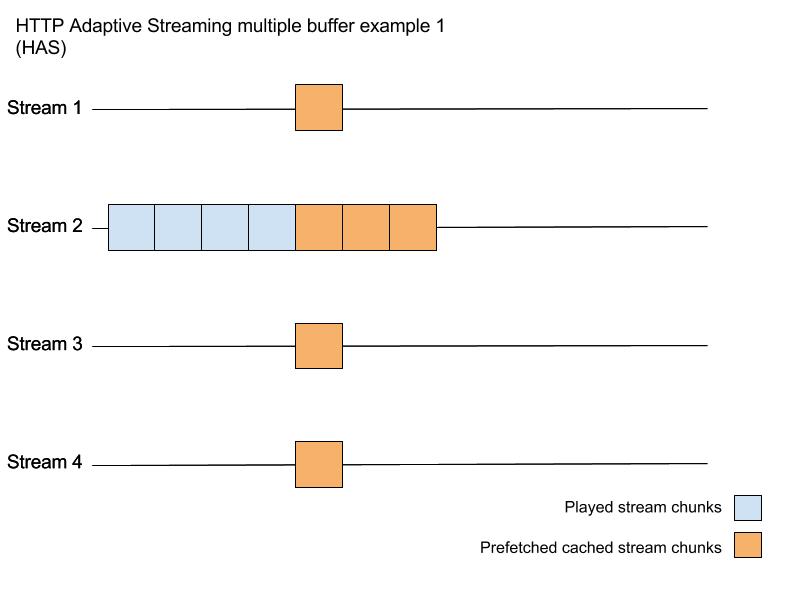
\includegraphics[scale=0.3]{HAS1.png}
\caption{HAS Parallell Stream Buffer 1}
\label{fig:HAS1}
\end{center}
\end{figure}

\begin{figure}[!ht]
\begin{center}
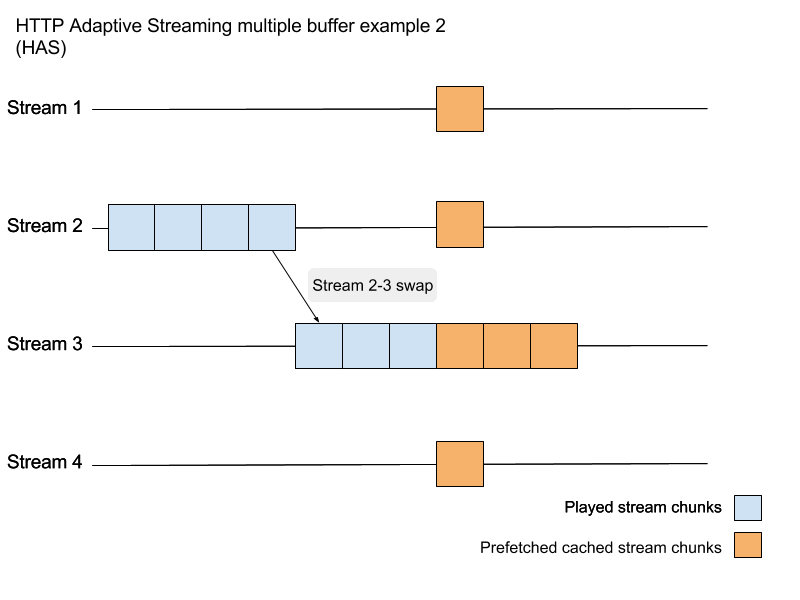
\includegraphics[scale=0.3]{HAS2.png}
\caption{HAS Parallell Stream Buffer 2}
\label{fig:HAS2}
\end{center}
\end{figure}

\subsection{Strobe Media Playback}

To display the stream in our application we will be using a media player called Strobe Media Playback (SMP), created with the Open Source Media Framework (OSMF) by Adobe Systems. The OSMF itself is build upon Adobe Flash Player, while becoming more outdated by day and discontinued by some, is widely used for media and other graphic applications and suffices to use for the proof-of-concept of our application. In practice this means that the media player is created using the tools that OSMF provides, compiled into a runnable flash file bytecode and run by Adobe Flash Player. 
OSMF supports a number of important features that will be used within our interface. Most importantly it enables the use of HAS with its HTTP streaming support and progressive downloading. It also enables the player to seamlessly switch between several media elements by using a composition of “nested serial elements”, which will be prominently used within our application.\cite{osmf}

\section{System Design}

To advance in this project we will mainly be programming, designing and developing the application. The programming language of choice will be Java Action Script and the IDE Flash Builder, which is very similar to the IDE Eclipse. The functionality of the interface to be developed is multiple. We want the interface to accept incoming video streams tagged with a location and cardinal direction from expected sources. The video streams will have to be tagged with these geographical datas somehow, which is not a common included feature with most video recording softwares. Developing a separate recording application to create these kind of video streams, for the sake of this project, might be outside of our goal of limitations for this project. If it is, we will prove the functionality of our interface with fabricated video geo-tags. These streams will then be made to work with the custom OSMF player.  Under-the-hood features will include HAS to ensure a smooth playback of the streams, both for buffering a single stream but also for prefetching and buffering a fraction of the other streams to ensure uninterrupted playback during stream swaps. To help us focus on the main problem of developing this interface, we are being provided with some existing code by our supervisors. This includes a working SMP player created with a modified version of OSMF with code from an existing HAS-interface using prefetching \cite{qualbranch}.

\subsection{Interface design}
The main part of this project is to expand upon the existing user interface (UI) of the default SMP player, as seen in Figure \ref{fig:mediaplayer}, and create a new section of it where we can implement the new desired functionality of this project. 

In practice we decided to go with adding an additional button to the control bar of the UI. When pressed, the graphical interface similar to the one in Figure \ref{fig:gpsinterface} is shown in the media player. Within this graphical interface, the user can hover over the arrows representing the available video streams located at different geographical locations and angles. While hovering over an arrow a tooltip is shown with some info about the video in question, such as GPS Coordinates and the angle, to give the user a comprehensive overview of the available streams. Finally, when an arrow is clicked the selected video is played with a seamless transition thanks to HAS.

The layout will also display a view of every stream and an optional “Point of interest” with its own geographical position. This point of interest is the center of all the different video streams and can be anything from a concert to some other large event. The added geographical view will also display the north, west, east and south cardinal directions to know the angle of the every stream relative to them. The angle $\theta$ in Figure \ref{fig:gpsinterface} can be calculated by taking the magnitude heading from a recording client. This will give us the direction relative to the north cardinal direction.

\subsection{Multipath???}

As mentioned briefly in section 2.1 chunks will be downloaded in a round-robin way and chunks will be downloaded only during the downtime of the HAS-player. Krishnamoorthi et al. \cite{bandawarePrefetch} mention a policy called \textit{best-effort} that we will use, in which chunks are only downloaded after the buffer size has reached $T_{max}$ and will start to prefetch chunks from several other videos. These chunks are only going to download as long as the time it takes to download them doesn't go below $T_{min}$ of the currently streamed video. The policy adapts to available bandwidth and varying network conditions. It is also one of the better policies discussed since it downloads chunks of as many videos as possible which is a needed and important functionality in  scenarios with many different streams \cite{bandawarePrefetch}. In Figure \ref{fig:prefetch} an idea of this can be seen. Other nearby streaming videos will only be downloaded ones $T_{max}$ is reached. A nearby video will be prefetched only in few chunks and the videos are downloaded in a round-robin way. Alternative video 1 followed by 2 and so on. Ones the $T_{min}$ is reached the main video is resumed downloading. The idea that would be best but will not be implemented is what video should be prefetched first or if that could be chosen. Prefetching distant videos may be better because they are probably more likely to be switched to. An interesting idea but not considered here for our proof-of-concept.

\begin{figure}[t!]
\begin{center}
	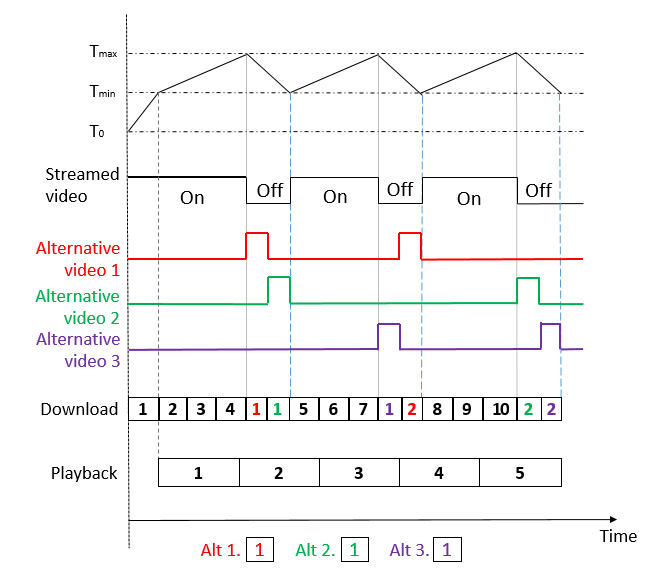
\includegraphics[scale=0.5]{prefetch.png}
	\caption{Prefetching overview}
	\label{fig:prefetch}
\end{center}
\end{figure}

\begin{figure}[t!]
\begin{center}
	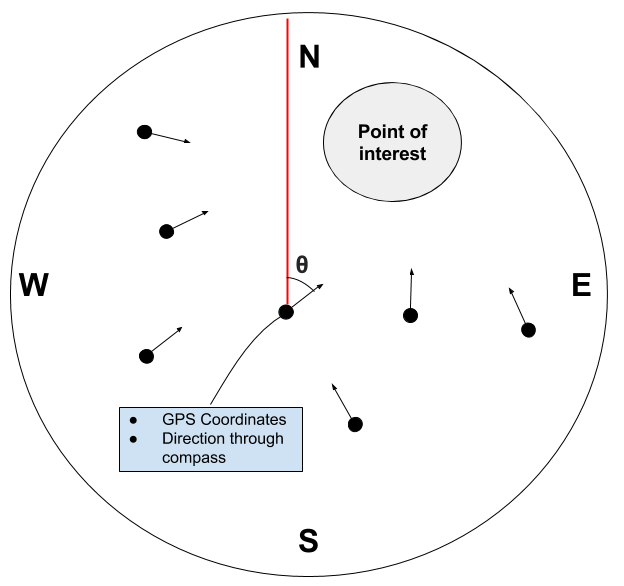
\includegraphics[scale=0.5]{teomet.png}
	\caption{Concept interface of GPS and Direction selection map}
	\label{fig:gpsinterface}
\end{center}
\end{figure}


The SMP player is by default set to play a stream of video located at a server supporting HTTP-streaming. For this project we'll be using the Adobe Media Server for enabling the chunked video streaming needed for our HAS functionality. Since we will be using a similar OSMF player that were used in Krishnamoorthi et al. \cite{hasmultipath}, the quality of our prefetched chunks will be adaptive to the available bandwidth. \cite{hasmultipath}.

\subsection{Relative placement of Geographical Points [PH]}
The interface accepts an arbitrary number of video streams coupled with a cardinal direction and GPS-coordinates, including latitude and longitude values. The graphical points representing these video streams with coordinates should then be placed and scaled relatively to eachother on the interface's geographical map. To accomplish this automatic placement and scaling we developed an algorithm to calculate where the points should be drawn to keep their relative positions between eachother, so the graphical points accurately represents the real life locations of the recordings.

XXXXXXX SKRIV HUR JONATHANS ALGORITM FUNGERAR XXXXXXX

\begin{figure}[t!]
\begin{center}
	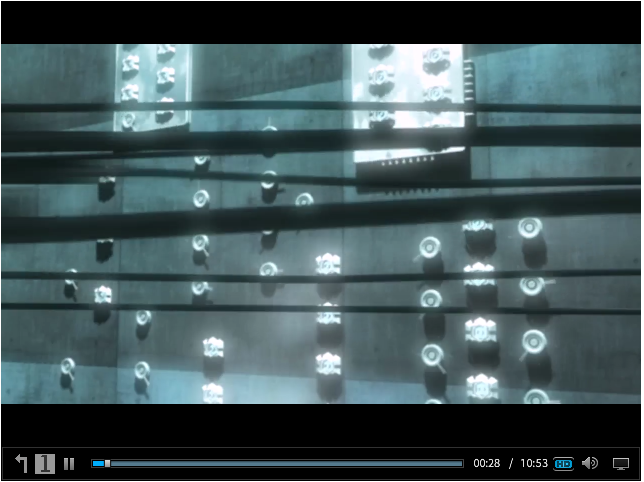
\includegraphics[scale=0.5]{Media_player.png}
	\caption{Strobe Media Player}
	\label{fig:mediaplayer}
\end{center}
\end{figure}

\section{Validated Result}
Testfall
Mätningar
Lite bilder där vi kör programmet med egna filmer


\section{Discussion}
Här prata om vilka svårigheter vi haft, vilka ändringar i planen vi gjorde från början till slutet, vad vi kompromissat med. Även att vi hoppade prefetching/överlämnade det jobbet till Vengeth?

\section{Conclusion}

%%För referering i flytande text till refereringen själv:
%%[Efternamnet på första författaren] et al. [citatnummer]

\clearpage
\begin{thebibliography}{9}

\bibitem{gtube}
  Jia Hao, Roger Zimmermann, Haiyang Ma,
  \emph{GTube: Geo-Predictive Video Streaming over HTTP in Mobile Environments}.
  \newline
  Published: 2014. Fetched: 2016-03-09 
  \newline
	URL: \text{http://goo.gl/6DiQiW}.

\bibitem{qualbranch}
  Vengatanathan Krishnamoorthi, Niklas Carlsson, Derek Eager, Anirban 
Mahanti, and Nahid Shahmehri,
  \emph{Quality-adaptive Prefetching for Interactive 
Branched Video using HTTP-based Adaptive Streaming}.
  \newline
  Proc. ACM 
International Conference on Multimedia (ACM Multimedia), Orlando, FL, Nov. 2014, pp. 317--326.

\bibitem{osmf}
  Greg Hamer,
  \emph{Open Source Media Framework: Introduction and overview}.
  \newline
  Published: 2010-03-15. Fetched: 2016-03-09
 \newline
  URL: http://www.wi-fiplanet.com/tutorials/article.php/3433451/Implementing-Wi-Fi-Multicast-Solutions.htm.
  
  \bibitem{streamrate}
  T. Huang, N. Handigol, B. Heller, N. McKeown, and R. Johari,
  \emph{Confused, timid, and unstable: Picking a video streaming rate is hard.}.
  \newline
  In Proc. ACM IMC (November 2012).
  
  \bibitem{hasmultipath}
  Vengatanathan Krishnamoorthi, Patrik Bergström, Niklas Carlsson, Derek 
Eager, Anirban Mahanti, and Nahid Shahmehri,
  \emph{Empowering the Creative User: 
Personalized HTTP-based Adaptive Streaming of Multi-path Nonlinear Video}.
  \newline
  Proc. ACM 
Proc. ACM SIGCOMM Workshop on Future Human-Centric Multimedia Networking 
(FhMN), Hong Kong, Aug. 2013, pp. 53--58.

\bibitem{bandawarePrefetch}
Vengatanathan Krishnamoorthi, Niklas Carlsson, Derek Eager, Anirban 
Mahanti, and Nahid Shahmehri,
	\emph{Bandwidth-aware Prefetching for Proactive 
Multi-video Preloading and Improved HAS Performance}.
	\newline
	Proc. ACM 
International Conference on Multimedia (ACM Multimedia), Brisbane, 
Australia, Oct. 2015.

\bibitem{scalableOnDemand}
Zhao, Y., D. L. Eager, and M. K. Vernon,
	\emph{Scalable On-Demand Streaming of 
Nonlinear Media}
	\newline
	 IEEE/ACM Trans. on Networking, Vol. 15, No. 5 (Oct. 
2007), pp. 1149-1162.

\bibitem{bufferbased}
T. Huang, R. Johari, and N. McKeown.
	\emph{ Downton abbey without the hiccups: Buffer-based rate adaptation for HTTP video streaming.}
	\newline
	 In Proc. ACM SIGCOMM FhMN
Workshop, Aug. 2013.


%\bibitem{randall2008}
%	Randall D. Knight,
%	\emph{Physics for Scientists and Engineers: A %Strategic Approach with Modern Physics (2nd %Edition)}.
%	\newline
%Addison-Wesley, 2a upplagan, 2008.

%\bibitem{polesAndZeros}

%	\emph{Understand Poles and Zeros}.
%	\newline
%	Publicerad 2002-11-01. Hämtat: 2015-06-01.
%	\newline
%	URL: http://web.mit.edu/2.14/www/Handouts/PoleZero.pdf

\end{thebibliography}

%%removes page number from this page
\thispagestyle{empty}

\end{document}
